\documentclass[10pt]{article}

\def\Type{LessonCaelan}
\def\TypeNum{Lesson 22}
\def\TypeTitle{Expectation and Variance}
\def\Semester{Fall 2021} %Not Used 
\def\Course{MATH 1190 \& 1210}

\usepackage{preambleDJ}




\begin{document}

\thispagestyle{firstpage}
\pagestyle{otherpages}
\vs{0.4}



\textbf{Intended Learning Outcomes}
After this lesson, you will be able to 

\begin{itemize}
    \item Define and explain the meaning of expectation and variance. (\target{P1, P2})
    \item Find the expectation and variance of a discrete random variable. (\target{P1})
    \item Find the expectation and variance of a continuous random variable. (\target{P2})
\end{itemize}

\vspace{-0.5cm}

\hrulefill

{\em What's the center of a data set?}. When we have a data set, frequently we want to determine what the ``middle" or ``center" of the set is.  For example, we might ask "What was the average score on Exam 1?", or "How much should I expect to pay in rent when I move to NY City?", or "What's Jose Altuve's batting average?"  These are all questions about the center of a given data set. Two ways to determine the center are:
\itemC{
\item Median
\item Mean (or Expected Value or Average).  {\em Notation} \blue{$\mu =E(X) = \bar{x}$}\\
}
We will use the terms {\em, mean}, {\em average} and {\em expected value} interchangeably.\\\\
\example{\target{P1}} \hs{-.2}\blue{\bf /}\blue{\bf\minil}{\bf Expected Value} (i.e. mean) of a roll of a 6 sided die. The average value when rolling a 6-sided die is \\
\mpageT{.65}{.35}{
\al{\mu=E(X)=\frac{1+2+3+4+5+6}{6}&=3.5\\\\
\frac{1}{6}+\frac{2}{6}+\frac{3}{6}+\frac{4}{6}+\frac{5}{6}+\frac{6}{6}&=3.5 \text{ \small (splitting apart the fraction)}\\\\
1\cdot \tikznode{nodeA1}{$\dfrac{1}{6}$}+2\cdot \tikznode{nodeB1}{$\dfrac{1}{6}$}+3\cdot \frac{1}{6}+4\cdot \frac{1}{6}+5 \cdot \frac{1}{6}+6\cdot \frac{1}{6}&=3.5 \text{ \small (pulling numerator out front of the fraction)}\\
}
}{\hs{-.75}
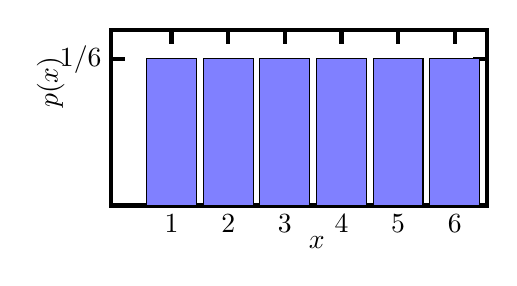
\begin{tikzpicture}
\begin{axis}[
x label style={anchor=west},
xlabel={$x$},
xtick       = {1,2,3,4,5,6},
%xticklabels = {$\$0$,$\$40$,$\$80$,$\$120$,$\$160$},
xticklabel style={anchor=north},
y label style={anchor=west},
ylabel={$p(x)$},
ytick={1/6},
yticklabels = {$1/6$},
enlarge x limits={.01}, % Adjusts spacing between bars and axis limits
samples     = 320,
xmin =0, xmax = 6.5,
ymin = 0, ymax = .2,
axis line style = { ultra thick, -},
every major tick/.append style={ultra thick, black, major tick length=5pt},
width=2.5in, height=1.5in
]
\addplot[ybar, bar shift=0,   bar width=18pt,  fill=blue!50] plot coordinates { (1,.167)  (2,0.167) (3,0.167) (4,0.167) (5,0.167)  (6,0.167) };
\end{axis}
\end{tikzpicture}
}
\vs{-.2}
\al{
&1\cdot \tikznode{nodeA2}{$P(X=1)$} +2\cdot \tikznode{nodeB2}{$P(X=2)$}+3\cdot P(X=3)+4\cdot P(X=4)+5\cdot P(X=5)+6\cdot P(X=6)=3.5\\\\
&1\cdot \tikznode{nodeA3}{$p(1)$} +2\cdot \tikznode{nodeB2}{$p(2)$}+3\cdot p(3) +4\cdot p(4)+5\cdot p(5)+6\cdot p(6)=3.5 \text{ \;\;\small (since $p(1)=P(X=1)$, etc.)}\\\\
&E(X)=
}
\vs{1} \\
 In general, if we have a random variable $X$ for a set of $n$ outcomes $\{x_1,x_2,x_3\dots,x_n\}$, the {\em  Expected Value}   (or {\em mean} or {\em average}) is 
 \importantV{Expected Value}{~\\
\parbox{4.5in}{ \hs{.6}$\mu=E(X)= $}\\ 
}


\newpage

\exercise\ltrm{\bf\color{Orange}P1} A fair coin whose sides are numbered ``$0$" and ``$1$" is flipped {\it three times}. If $X$ represents the sum of the outcome of each flip, then the PMF of $X$ and histogram are below.  Find $\mu=E[X]$ by using the equation we developed on the previous page.\\
\hs{-.3}\mpageTth{.3}{.35}{.35}[][\hs{-.4}]{
\[ p(x)=\begin{cases}
\frac18 & \text{when }x=0\\
\frac38 & \text{when }x=1\\
\frac38 & \text{when }x=2\\
\frac18 & \text{when }x=3\\
0 & \text{otherwise}
\end{cases}\]
}{
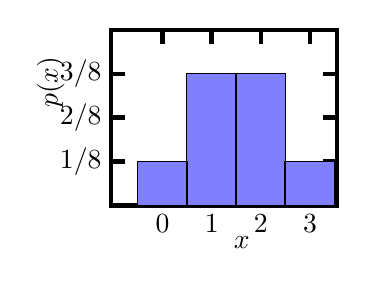
\begin{tikzpicture}
\begin{axis}[
x label style={anchor=west},
xlabel={$x$},
xtick       = {1,2,3,4},
xticklabels = {$0$,$1$,$2$,$3$},
xticklabel style={anchor=north},
y label style={anchor=west},
ylabel={$p(x)$},
ytick={1/8,1/4,3/8},
yticklabels = {$1/8$,$2/8$, $3/8$},
enlarge x limits={.01}, % Adjusts spacing between bars and axis limits
samples     = 320,
xmin =0, xmax = 4.5,
ymin = 0, ymax = .5,
axis line style = { ultra thick, -},
every major tick/.append style={ultra thick, black, major tick length=5pt},
width=1.75in, height=1.5in
]
\addplot[ybar, bar shift=0,   bar width=18pt,  fill=blue!50] plot coordinates { (1,0.125)  (2,0.375) (3,0.375) (4,0.125) };
\end{axis}
\end{tikzpicture}
}{
%
}
\vs{.5}~\\
{\bf Variance} {\em How do we determine how much data is scattered?} Let's look at two different data sets. The first data set represents the height of houses that a conservative builder builds. She takes a conservative approach and thus builds all the houses the same.  The second data set represents the height of houses  a speculative builder builds in an attempt to create more interest and income.   
\graphicsC{buildingHeights}{5.5}
\example{\target{P1}}
We let $C$ be a random variable associated with heights of buildings from the conservative builder and $S$ a random variable associated with the heights of buildings from the speculative builder. The probability to build each building  is equally likely for each builder (i.e. $p(x)=\dfrac{1}{5}$).  
\tasksA{2}{
\task Find $\mu=E(C)$

\task {\em Attempt $\#1$} What is the average amount each building height differs from $\mu$ for the conservative builder?\vs{1}

\task Find $\mu=E(C)$

\task {\em Attempt $\#1$} What is the average amount each building height differs from $\mu$ for the speculative builder?
}
\newpage
\tasksAS{2}{5}{
\task* {\em Attempt $\#2$} {\em Hint: }Force the differences to be positive. We're going to call this new approach the  {\em variance} with notation $Var(X)$.
\vs{1.5}
}
 \footnotetext{It is possible  to take the absolute value of each  difference to make the positive.  This approach is called {\em Mean Absolute Error} (MAE).  However, the most commonly used approach in statistics is to square the difference.  }
\vs{1}
{\em Key Idea: Variance is} 

\vs{2.5}~\\
\exercise\ltrm{\bf\color{Orange}P1} A fair coin whose sides are numbered ``$0$" and ``$1$" is flipped {\it three times}. If $X$ represents the sum of the outcome of each flip, then the PMF of $X$ and histogram are below.  Find $Var(x)$ using $\mu$ from previous exercise..\\
\hs{-.5}\mpageTth{.25}{.3}{.35}[][\hs{-.2}]{
\[ p(x)=\begin{cases}
\frac18 & \text{when }x=0\\
\frac38 & \text{when }x=1\\
\frac38 & \text{when }x=2\\
\frac18 & \text{when }x=3\\
0 & \text{otherwise}
\end{cases}\]
}{
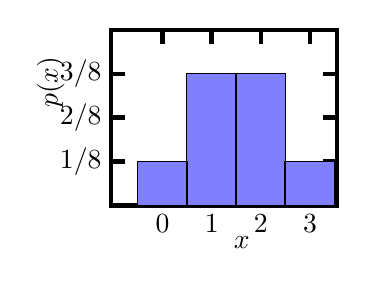
\begin{tikzpicture}
\begin{axis}[
x label style={anchor=west},
xlabel={$x$},
xtick       = {1,2,3,4},
xticklabels = {$0$,$1$,$2$,$3$},
xticklabel style={anchor=north},
y label style={anchor=west},
ylabel={$p(x)$},
ytick={1/8,1/4,3/8},
yticklabels = {$1/8$,$2/8$, $3/8$},
enlarge x limits={.01}, % Adjusts spacing between bars and axis limits
samples     = 320,
xmin =0, xmax = 4.5,
ymin = 0, ymax = .5,
axis line style = { ultra thick, -},
every major tick/.append style={ultra thick, black, major tick length=5pt},
width=1.75in, height=1.5in
]
\addplot[ybar, bar shift=0,   bar width=18pt,  fill=blue!50] plot coordinates { (1,0.125)  (2,0.375) (3,0.375) (4,0.125) };
\end{axis}
\end{tikzpicture}
}{
%
}


\newpage
\blue{\bf Summary: Expectation \& Variance of Discrete Random Variables}\\
\mpageT{.5}{.5}{
\importantV{Expected Value}{$\mu=E[X] = \displaystyle\sum_{i=1}^n x_i\cdot p(x_i)$} 
}{
\importantV{Variance}{\vs{-.1}
\enum{
\item $\ds Var(X) = E[(X-\mu)^2]\sum_{i=1}^n(x_i-\mu)^2p(x_i)$
\item $\ds Var(X)=E[X^2]-\mu^2= \left(\sum_{i=1}^n (x_i)^2\cdot p(x_i)\right)-\mu^2$
}
}
}


\exercise\ltrm{\bf\color{Orange}P1} Histograms representing the PMFs of random variables $X_1$, $X_2$, and $X_3$ (respectively) are given below.\vs{-.2}\\

\mpageTth{.33}{.33}{.33}{
\begin{center}
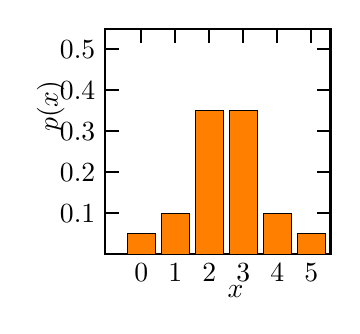
\begin{tikzpicture}
\begin{axis}[
x label style={anchor=west},
xlabel={$x$},
xtick       = {1,2,3,4,5,6},
xticklabels = {$0$,$1$,$2$,$3$, $4$, $5$},
xticklabel style={anchor=north},
y label style={anchor=west},
ylabel={$p(x)$},
ytick={0.1,0.2,0.3,0.4, 0.5},
%yticklabels = {$1/8$,$2/8$, $3/8$},
enlarge x limits={.01}, % Adjusts spacing between bars and axis limits
samples     = 320,
xmin =0, xmax = 6.5,
ymin = 0, ymax = .55,
axis line style = {  thick, -},
every major tick/.append style={ thick, black, major tick length=5pt},
width=1.75in, height=1.75in
]
\addplot[ybar, bar shift=0,   bar width=10pt,  fill=orange] plot coordinates { (1,0.05)  (2,0.1) (3,0.35) (4,0.35) (5,0.1) (6,0.05) };
%\draw[red, dashed] (3.5,-.1)--(3.5,.48);
%\node[red] at (3.5,.5) {$\mu=2.5$};
\end{axis}
\end{tikzpicture}
\parbox{1.15\textwidth}{\captionof*{figure}{Histogram for $X_1$}}
\end{center}
%
%
}{
\begin{center}
 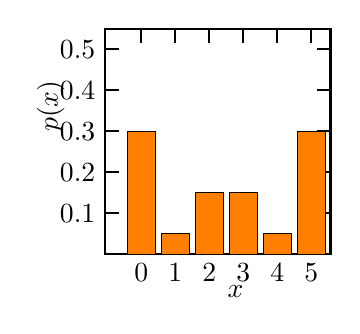
\begin{tikzpicture}
\begin{axis}[
x label style={anchor=west},
xlabel={$x$},
xtick       = {1,2,3,4,5,6},
xticklabels = {$0$,$1$,$2$,$3$, $4$, $5$},
xticklabel style={anchor=north},
y label style={anchor=west},
ylabel={$p(x)$},
ytick={0.1,0.2,0.3,0.4, 0.5},
%yticklabels = {$1/8$,$2/8$, $3/8$},
enlarge x limits={.01}, % Adjusts spacing between bars and axis limits
samples     = 320,
xmin =0, xmax = 6.5,
ymin = 0, ymax = .55,
axis line style = {  thick, -},
every major tick/.append style={ thick, black, major tick length=5pt},
width=1.75in, height=1.75in
]
\addplot[ybar, bar shift=0,   bar width=10pt,  fill=orange] plot coordinates { (1,0.3)  (2,0.05) (3,0.15) (4,0.15) (5,0.05) (6,0.3) };
%\draw[red, dashed] (3.5,-.1)--(3.5,.48);
%\node[red] at (3.5,.5) {$\mu=2.5$};
\end{axis}
\end{tikzpicture}
\parbox{1.15\textwidth}{\captionof*{figure}{Histogram for $X_2$}}
\end{center}
%
%
}{
\begin{center}
 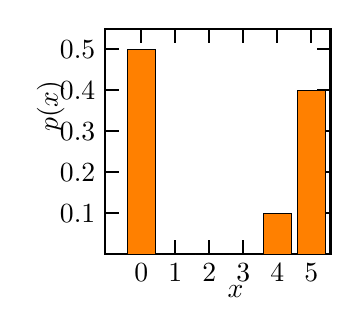
\begin{tikzpicture}
\begin{axis}[
x label style={anchor=west},
xlabel={$x$},
xtick       = {1,2,3,4,5,6},
xticklabels = {$0$,$1$,$2$,$3$, $4$, $5$},
xticklabel style={anchor=north},
y label style={anchor=west},
ylabel={$p(x)$},
ytick={0.1,0.2,0.3,0.4, 0.5},
%yticklabels = {$1/8$,$2/8$, $3/8$},
enlarge x limits={.01}, % Adjusts spacing between bars and axis limits
samples     = 320,
xmin =0, xmax = 6.5,
ymin = 0, ymax = .55,
axis line style = {  thick, -},
every major tick/.append style={ thick, black, major tick length=5pt},
width=1.75in, height=1.75in
]
\addplot[ybar, bar shift=0,   bar width=10pt,  fill=orange] plot coordinates { (1,0.5)  (2,0) (3,0) (4,0) (5,0.1) (6,0.4) };
%\draw[red, dashed] (3.4,-.1)--(3.4,.48);
%\node[red] at (3.4,.5) {$\mu=2.4$};
\end{axis}
\end{tikzpicture}
\parbox{1.15\textwidth}{\captionof*{figure}{Histogram for $X_3$}}
\end{center}
}{
}
\vs{-.2}
\enumA{
\item Before computing anything and basing your answer solely on the PMF above, put the variances of the three random variables in order from least to greatest. Explain your reasoning.

\vs{2.5}

\item Sketch an example of a histogram representing the PMF of a random variable $Y$ having {\bf higher} variance than $X_3$. Sketch an example of a histogram representing the PMF of a random variable $Z$ having the same mean as $X_1$ but {\bf lower} variance than $X_1$.\vs{-.15}\\
\mpageT{.5}{.5}{
\centering
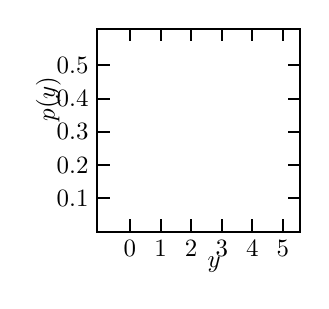
\begin{tikzpicture}[scale=0.9]
\begin{axis}[
x label style={anchor=west},
xlabel={$y$},
xtick       = {1,2,3,4,5,6},
xticklabels = {$0$,$1$,$2$,$3$, $4$, $5$},
xticklabel style={anchor=north},
y label style={anchor=west},
ylabel={$p(y)$},
ytick={0.1,0.2,0.3,0.4, 0.5},
%yticklabels = {$1/8$,$2/8$, $3/8$},
enlarge x limits={.01}, % Adjusts spacing between bars and axis limits
samples     = 320,
xmin =0, xmax = 6.5,
ymin = 0, ymax = .61,
axis line style = {  thick, -},
every major tick/.append style={ thick, black, major tick length=5pt},
width=1.75in, height=1.75in
]
%\addplot[ybar, bar shift=0,   bar width=10pt,  fill=orange] plot coordinates { (1,0.5)  (2,0) (3,0) (4,0) (5,0) (6,0.5) };
%\draw[red, dashed] (3.5,-.1)--(3.5,.58);
%\node[red] at (3.5,.58) {$\mu=2.5$};
\end{axis}
\end{tikzpicture}
}{
\centering
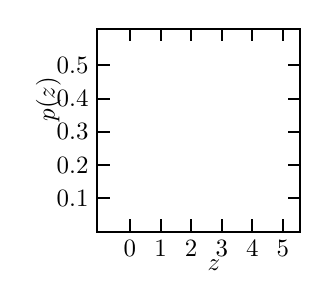
\begin{tikzpicture}[scale=0.9]
\begin{axis}[
x label style={anchor=west},
xlabel={$z$},
xtick       = {1,2,3,4,5,6},
xticklabels = {$0$,$1$,$2$,$3$, $4$, $5$},
xticklabel style={anchor=north},
y label style={anchor=west},
ylabel={$p(z)$},
ytick={0.1,0.2,0.3,0.4, 0.5},
%yticklabels = {$1/8$,$2/8$, $3/8$},
enlarge x limits={.01}, % Adjusts spacing between bars and axis limits
samples     = 320,
xmin =0, xmax = 6.5,
ymin = 0, ymax = .61,
axis line style = {  thick, -},
every major tick/.append style={ thick, black, major tick length=5pt},
width=1.75in, height=1.75in
]
%\addplot[ybar, bar shift=0,   bar width=10pt,  fill=orange] plot coordinates { (1,0)  (2,0) (3,0.5) (4,0.5) (5,0) (6,0) };
%\draw[red, dashed] (3.5,-.1)--(3.5,.58);
%\node[red] at (3.5,.58) {$\mu=2.5$};
\end{axis}
\end{tikzpicture}
}
}
%\vs{-.5}
%\sol{
%\itemI{
%\item %If $P(X=0)=0.5$ and $P(X=5)=0.5$ $\mu=E(X)=0\cdot 0.5+5\cdot 0.4=2.5$. 
%$Var(Y)>Var(X_3)$ because there our only two outcomes ($X=0$ and $X=5$) and these are furtherest from the center, $\mu=2.5$ while $X_3$ has an additional outcome ($X=4$) that is closer to the center at $\mu$.
%\item $Var(Z)<Var(X_1)$ since there are only two outcomes ($X=2$, $X=3$ and these are closes to the center , $\mu=2.5$ while $X_1$ has additional out comes that are farther from $\mu$.
%}
%}
\begin{center}
({\bf Note:} don't forget that the total probability must be exactly 1.)
\end{center}
\hfill

\newpage
%%%%%%%%%
%%%%%%%%%
%%%%%%%%%
%%%%%%%%%
\label{page1}
\blue{\bf Key Properties of  Continuous Random Variables}\\
\mpageT{.5}{.5}[\hs{.1}]{
\centering
\blue{ \bf Discrete Random Variables}
}{
\centering
\blue{ \bf Continuous Random Variables}\\
}%\vs{-.2}
\itemNIN{
\mpageT{.5}{.5}[\hs{.2}]{
\item {\bf Discrete Example: } The random variable $X$ is the sum from randomly rolling two $4$-sided dice
}{
\item {\bf Continuous Example } The random variable $T$ is the (random) wait time until the bus arrives  at the 
amphitheater on McIntyre. Buses arrive every $30$ minutes with evenly distributed probability (a uniform distribution)
}
\\
\mpageT{.5}{.5}[\hs{.2}]{
\item The {\em Sample Space of $X$}: $S_X=\{2,3,4,5,6,7,8\}$
}{
\item The {\em Support of $T$}: $S_T=$  $[a,b]=[0,30]$  or $0\leq t\leq 30$
}

\mpageT{.5}{.5}[\hs{.2}]{
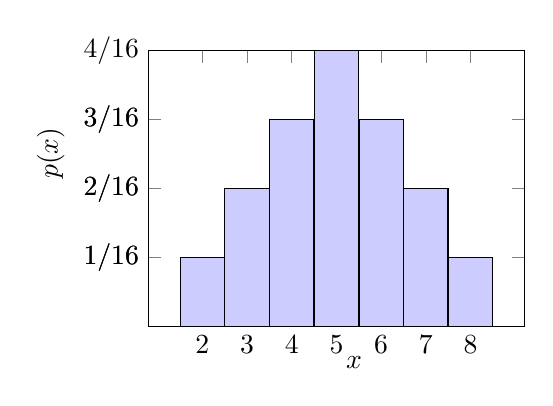
\begin{tikzpicture}
\begin{axis}[
	xtick={1,	2,	3,	4,	5,	6,	7}, % Places x-axis ticks at data points
	xticklabels={
         2,	3,	4,	5,	6,	7,	8
         }, % Custom x-axis labels
ytick       = {1/16, 2/16, 3/16,4/16,3/16,2/16,1/16},
yticklabels =  {$1/16$, $2/16$, $3/16$,$4/16$,$3/16$,$2/16$,$1/16$},
enlarge x limits={.2}, % Adjusts spacing between bars and axis limits
	y label style={anchor=south west},
	ylabel={$p(x)$},
	xlabel = {$x$},
	x label style={anchor=west},
	%xticklabel style = {font=\small}, 
	ymin = 0, ymax = .25,
	width = 2.5in, height=2in,
	   axis line style={->},
]
\addplot[ybar, bar shift=0,   bar width=16pt,  fill=blue!20] plot coordinates {
(1,.0625)  (2,.125) (3,.1875) (4,.25) (5,.1875) (6,.125) (7,.0625) 
};
\end{axis}
\end{tikzpicture}
}{
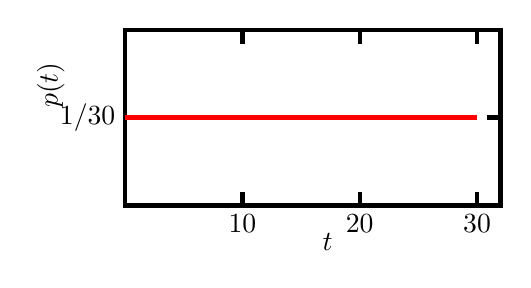
\begin{tikzpicture}
\begin{axis}[
	x label style={anchor=west},
xlabel={$t$},
xtick       = {10,20,30},
%xticklabels = {$10$,$20$,$30$},
xticklabel style={anchor=north},
y label style={anchor=west},
ylabel={$p(t)$},
%ytick=\empty,
%ytick       = {1/30},
ytick={0.05},
yticklabels = {$1/30$},
samples     = 320,
xmin =0, xmax = 32,
ymin = 0, ymax = .1,
axis line style = { ultra thick, -},
every major tick/.append style={ultra thick, black, major tick length=5pt},
width=2.5in, height=1.5in
]
  \addplot[domain=0:30, red, ultra thick, mark=none]{.05};
\end{axis}
\end{tikzpicture}
%
%
%~\\\blue{Note that the support of a Continuous Random Variable (RV) will be an interval of the form\\ $a\leq t\leq b=[a,b]$}
}
~\\
\mpageT{.5}{.5}[\hs{.2}]{
\item {\bf Probability Mass Function}:  $p(x)$.\\
{ \em Two Properties:}
\enum{
\item $0\leq p(x)\leq 1$ where $x\in S_X$\vs{.3}
\item $\ds \sum_{k\in S_X}P[X=k] = \sum_{k=2}^8 P[X=k]=\sum_{k=2}^8 p(k)=1$
}
%
}{
\item {\bf Probability Density Function (PDF)}: $p(t)$.\\
{ \em Two Properties:}
\enum{
\item $p(t)\geq0$ where $t\in S_T$. Note that this differs from discrete random variables in that there is {\em not} a requirement that $p(t)\leq 1$.
\item $\ds \int_a^b p(t)\;dt=\ds \int_0^{30} p(t)\;dt=1$ 
}
\vs{-.1}~\\
}
\mpageT{.5}{.5}[\hs{.2}]{
\item {\bf Cumulative Probability} $\ds P(X\leq 4)=\sum_{k=2}^4 p(k)$ \\
%
%
}{
\item {\bf Cumulative Probability:}  $P\ds (T\leq 10)= \int_0^{20}p(t)\;dt$
%
}\vs{-.3}\\
\mpageT{.5}{.5}[\hs{.2}]{
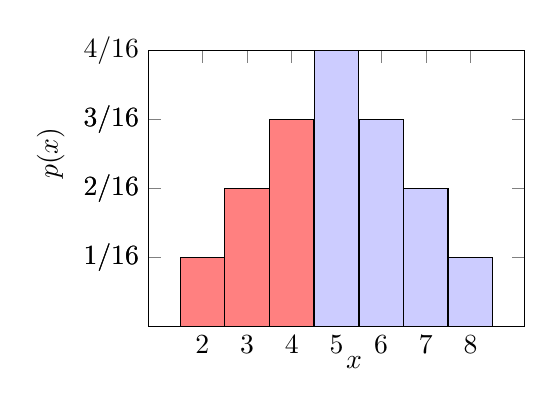
\begin{tikzpicture}
\begin{axis}[
	xtick={1,	2,	3,	4,	5,	6,	7}, % Places x-axis ticks at data points
	xticklabels={
         2,	3,	4,	5,	6,	7,	8
         }, % Custom x-axis labels
ytick       = {1/16, 2/16, 3/16,4/16,3/16,2/16,1/16},
yticklabels =  {$1/16$, $2/16$, $3/16$,$4/16$,$3/16$,$2/16$,$1/16$},
enlarge x limits={.2}, % Adjusts spacing between bars and axis limits
	y label style={anchor=south west},
	ylabel={$p(x)$},
	xlabel = {$x$},
	x label style={anchor=west},
	%xticklabel style = {font=\small}, 
	ymin = 0, ymax = .25,
	width = 2.5in, height=2in,
	   axis line style={->},
]
\addplot[ybar, bar shift=0,   bar width=16pt,  fill=blue!20] plot coordinates { (1,.0625)  (2,.125) (3,.1875) (4,.25) (5,.1875) (6,.125) (7,.0625) };
\addplot[ybar, bar shift=0,   bar width=16pt,  fill=red!50] plot coordinates { (1,.0625)  (2,.125) (3,.1875)  };
\end{axis}
\end{tikzpicture}
}{
\begin{tikzpicture}
\begin{axis}[
	x label style={anchor=west},
xlabel={$t$},
xtick       = {10,20,30},
%xticklabels = {$10$,$20$,$30$},
xticklabel style={anchor=north},
y label style={anchor=west},
ylabel={$p(t)$},
%ytick=\empty,
%ytick       = {1/30},
ytick={0.05},
yticklabels = {$1/30$},
samples     = 320,
%domain      = -2.5:2.5,
%restrict y to domain=-6.5:6.5,
xmin =0, xmax = 32,
ymin = 0, ymax = .1,
axis line style = { ultra thick, -},
every major tick/.append style={ultra thick, black, major tick length=5pt},
width=2.5in, height=1.5in
%  grid=both, grid style=solid
]
 \addplot[name path=f, domain=0:30, red, ultra thick, mark=none]{.05};
 %\addplot[ name path=f, domain=0:26,  red, ultra thick, <->, ] {1/sqrt(2*pi*(3.85)^2)*e^(-(x-13.5)^2/(2*(3.85)^2))  };
	   \path[name path=axis] (0,0) -- (10,0);
	    \addplot [
thick,
color=red,
fill=red, 
fill opacity=0.35
]
fill between[
of=f and axis,
soft clip={domain=0:10},
];
ne]{-1/25*x+2/5};
\end{axis}
\end{tikzpicture}
~\\\\
%
%
%\blue{Cumulative probability for Discrete RVS is represented by areas of histogram bars. Cumulative probability for Continuous RVs is also represented by (net) area and is thus computed via a definite integral instead of a sum.
%}
}
%\vs{.1}
\mpageT{.5}{.5}[\hs{.2}]{
\item {\bf Expected Value}  \\
$\ds \mu= E[X]=\sum_{i=1}^n x_i\cdot p(x_i)=\sum_{k=2}^8k\cdot p(k)$
%
%
}{
\item {\bf Expected Value:}  \\
$\ds \mu=E[T]=$ 
}
\mpageT{.5}{.5}[\hs{.2}]{
\item {\bf Variance}    (for $n$ outcomes)\vs{-.15}
\al{ Var(X)&=E[(X-\mu)^2]=\sum_{i=1}^n (x_i-\mu)^2p(x_i)\\
&=E[X^2]-\mu^2=\left(\sum_{i=1}^n x_i^2\cdot p(x)\right)-\mu^2
}
%
%
}{
\item {\bf Variance}\vs{.15}\\
%\al{
$Var(T)=E[(T-\mu)^2]=$\vs{.25}\\
\hs{.45}$=E[T^2]-\mu^2=$
}
}

%\newpage

\blue{\bf Summary of Expectation \& Variance of Continuous Random Variables}\\
\mpageT{.5}{.5}{
\importantV{Expected Value}{$\mu=E[X] = \displaystyle\int_a^b x\cdot p(x)\,dx$}
}{
\importantV{Variance}{
\enum{
\item $ \ds Var(X) = E[(X-\mu)^2]=\int_a^b(x-\mu)^2\cdot p(x)\;dx$
\item $\ds Var(X)=E[X^2]-\mu^2=\displaystyle\int_a^b x^2\cdot p(x)\,dx-\mu^2$
}
}
}



\exercise\ltrm{\bf\color{Orange}P2} Let the continuous random variable $V$ have the following PDF:\\
\mpageT{.5}{.5}{
\[
p(v) = 
\begin{cases} 
\dfrac{1}{v} & \text{for } 1 \leq v \leq e, \\
0 & \text{otherwise}.
\end{cases}
\]
}{
\begin{tikzpicture}
\begin{axis}[
	x label style={anchor=west},
xlabel={$v$},
xtick       = {1,2.72},
xticklabels = {$1$,$e$},
xticklabel style={anchor=north},
y label style={anchor=west},
ylabel={$p(v)$},
%ytick=\empty,
%ytick       = {1/30},
ytick={1},
yticklabels = {$1$},
samples     = 320,
xmin =0, xmax = 3,
ymin = 0, ymax = 1.3,
axis line style = { ultra thick, -},
every major tick/.append style={ultra thick, black, major tick length=5pt},
width=2.5in, height=1.5in
]
 \addplot[name path=f, domain=1:2.7182, blue, ultra thick, mark=none]{1/x};
\end{axis}
\end{tikzpicture}
}
\begin{itemize}
\item[(a)] Find the mean of $V$ using the definition of mean.  \vs{2}




\item[(b)] Find the variance of $V$ using one of the definitions of variance.


\end{itemize}

\newpage
\exercise\ltrm{\bf\color{Orange}P2} The integral $\dint_1^{c} \frac12z\,dz$ represents the expected value of a random variable $Z$, where $c$ is a constant to be determined.\\

\tasksA{2}{
\task Identify the PDF of $Z$.

\task Find the value of $c$. \vs{2.5}


\task Find the mean $\mu=E(Z)$

\task Find the variance of $Z$.



}

%%%%%%%%%
\newpage%
%%%%%%%%%

{\bf\color{blue}Extra Practice 1.}\ltrm{{\bf\color{Orange}P1}}
Let $X$ be a discrete random variable with the following probability mass function $p(x)$.

\begin{table}[h!]
        \centering
        \begin{tabular}{c|ccccc}
            \hline
           $x$  & 1 & 2 & 3 & 4 & 5\\
           \hline\\
           $p(x)$  & $\dfrac{3}{10}$ & $\dfrac{1}{10}$ & $\dfrac{1}{10}$ &\mbox{\hs{.25}} & $\dfrac{3}{10}$\\\\
           \hline
        \end{tabular}
    \end{table}

\begin{enumerate}
    \item[(a)] Find the missing value in the table so that $p(x)$ is a valid probability mass function. \vs{1.5}


    \item[(b)] Find the expected value of $X$.\vs{1.5}



    \item[(c)] Find the variance of $x$.

    \vfill
\end{enumerate}

%%%%%%%%%
\newpage%
%%%%%%%%%

{\bf\color{blue}Extra Practice 2.}\ltrm{{\bf\color{Orange}P2}}
Compute the expectation of a continuous random variable $W$ with PDF given by:
\[
p(w) = 
\begin{cases} 
2\sqrt{w} & \text{for } 0 \leq w \leq 1, \\
0 & \text{otherwise}.
\end{cases}
\]

\vs{2.5}

{\bf\color{blue}Extra Practice 3.}\ltrm{{\bf\color{Orange}P2}} 
Let $X$ be a continuous random variable with the following PDF and its graph.\\
\mpageT{.5}{.5}{\centering
\[
p(x) = 
\begin{cases} 
\dfrac{1}{x\ln(10)} & \text{for } 1 \leq x \leq 10, \\
0 & \text{otherwise}.
\end{cases}
\]
}{\centering
\begin{tikzpicture}
\begin{axis}[
	x label style={anchor=west},
xlabel={$x$},
xtick       = {1,10},
xticklabels = {$1$,$10$},
xticklabel style={anchor=north},
y label style={anchor=west},
ylabel={$p(x)$},
%ytick=\empty,
%ytick       = {1/30},
ytick={0.5},
%yticklabels = {$1$},
samples     = 320,
xmin =0, xmax = 10.5,
ymin = 0, ymax = 0.6,
axis line style = { ultra thick, -},
every major tick/.append style={ultra thick, black, major tick length=5pt},
width=2.5in, height=1.5in
]
 \addplot[name path=f, domain=1:10, blue, ultra thick, mark=none]{1/(x*ln(10)};
\end{axis}
\end{tikzpicture}
}
\tasksA{2}{
    \task Compute the expectation $\mu=E[X]$.

   \task Determine the variance $\text{Var}(X)$. 

   
}


\end{document}
%%%%%%%%%%%% END DOCUMENT %%%%%%%%%%%%%%%
